\documentclass[12pt]{article}

\usepackage{graphicx,color,enumerate,multicol}
\usepackage[top=1in, bottom=1in, left=1.25in, right=1.25in]{geometry}
\usepackage{tikz,pgfplots}

%% Use Minion fonts if available.  Otherwise Times.
\IfFileExists{MinionPro.sty}{\usepackage[lf]{MinionPro}}{}
\usepackage{amsmath,amsthm,amsbsy}
\IfFileExists{MinionPro.sty}{}{\usepackage{times,txfonts}}

%% Setup aproblem environment, 
%% aproblem items
%% subproblems environment
%% subproblem items
\makeatletter
\newcounter{probcount}
\newcounter{subprobcount}
\newlength\probsep
\newlength\pshrinking
\newif\iffirstprob
\newenvironment{aproblems}%
  {\ifhmode\unskip\par\fi\setcounter{probcount}{0}\probsep\parskip
  \sbox\@tempboxa{\textbf{9.}}\pshrinking\wd\@tempboxa\advance\pshrinking\labelsep
  \let\hproblem\aproblem
  \advance\linewidth -\pshrinking
  \advance\@totalleftmargin\pshrinking
  \advance\leftskip\pshrinking}%
  {\ifhmode\unskip \par\fi\advance\leftskip-\pshrinking}%

\newcommand{\aproblem}{%
  \setcounter{subprobcount}{0}%
  \stepcounter{probcount}%
  \def\@currentlabel{\arabic{probcount}}%
  \ifhmode
    \unskip \par
  \fi
%  \addpenalty{-4000}%
  \iffirstprob\else\addvspace\probsep\fi
  \firstprobfalse
  \hskip -\labelwidth\hskip -\labelsep 
  \hbox to\labelwidth{\hss\textbf{\arabic{probcount}.}}\hskip\labelsep
}%

% Use \begin{subproblems}\item...\item...\end{subproblems}
\renewcommand{\emph}[1]{\textsf{\textbf{#1}}}
\newenvironment{subproblems}{%
\begin{enumerate}%
\setcounter{enumi}{\value{subprobcount}}%
\renewcommand{\theenumi}{\emph{\alph{enumi}}}}%
{\setcounter{subprobcount}{\value{enumi}}\end{enumerate}}


%% The following commands put defined left and right headers on the top, and a page number
%% on the bottom of all pages beyond page 1
\usepackage{fancyhdr}
\pagestyle{fancy}
\fancyfoot[C]{\ifnum \value{page} > 1\relax\thepage\fi}
\fancyhead[L]{\ifx\@doclabel\@empty\else\@doclabel\fi}
\fancyhead[R]{\ifx\@docdate\@empty\else\@docdate\fi}
\headheight 15pt
\def\doclabel#1{\gdef\@doclabel{#1}}
\def\docdate#1{\gdef\@docdate{#1}}
\makeatother

%% General formatting parameters
\parindent 0pt
\parskip 6pt plus 1pt

\let\ds\displaystyle
\doclabel{Math F251: Midterm 2 Review}
\docdate{8 April 2019}


\begin{document}
\begin{aproblems}

\aproblem Consider the function $f(x)$ and its derivatives:
\begin{equation*}
\begin{aligned}
f(x)&=\frac{e^x}{1+x}\\
f'(x)&=\frac{xe^x}{(1+x)^2}\\
f''(x) &= \frac{e^x(x^2+1)}{(1+x)^3}.
\end{aligned}
\end{equation*}
\begin{subproblems}
\item Find the critical numbers of $f(x).$
\vfill
\item Find the open intervals on which the function is increasing or
    decreasing.
\vfill
\item Find the open intervals on which the function is concave up or
    concave down.  
\vfill
\newpage
\item Classify all critical points -- using the first derivative test.
\vfill
\item Classify all critical points -- using the second derivative test.
\vfill
\item Find the inflection points.
\vfill
\item Sketch the graph.
\vfill
\end{subproblems}
\newpage
\aproblem Find the linearization of $f(x)=\sqrt{x}$ at $a=4$ and use it to estimate $\sqrt{4.1}.$
\vfill
\aproblem  Show that the point $(2,3)$ lies on the curve $x^2+xy-y^2=1$.
Then find the slope of the tangent line to the curve at that point.
\vfill

\newpage
\aproblem 
A ball of metal is being heated in an oven, and its radius is increasing
at a rate of $0.1$ cm/min.  At what rate is the ball's volume increasing
when its radius is $3$ cm?
\vfill
%lhop

\aproblem Evaluate the following limits.

$\displaystyle\lim_{x \to 0} \frac{1+x- e^x}{\sin x}$\hfill
$\lim_{x \to 0^+} (1+2x)^{1/x}$\hfill\strut
\vfill

\newpage
%page 5
\aproblem A landscape architect wishes to enclose a rectangular garden on
one side by a brick wall costing \$30 per foot and on the
other three sides with a metal fence costing \$10 per foot.
The area of the garden is to be 800ft$^2$.  What
are the dimensions of the garden that minimize the cost of the fencing?

\hfil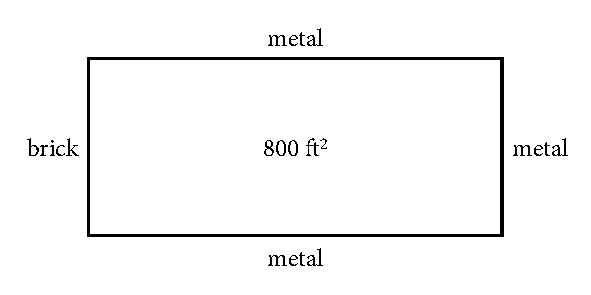
\includegraphics{FinalOptimize}

\vfill
\newpage
%Mean Value Theorem
\aproblem
\begin{subproblems}
\item State the Mean Value Theorem and draw a picture to illustrate it.
\vspace{2in}
\item Suppose $f(x)$ is continuous on $[-1,1]$ and has a derivative
at each $x$ in $(-1,1)$.  If $f(-1)=7$ and $f(1)=5$, what does
the Mean Value Theorem let you conclude?
\end{subproblems}
\vfill
\end{aproblems}
\end{document}
